\chapter{Results}
\label{chp:results}

This chapter is split into three sections, emphasizing the game-theoretical solution results in the first section and the simulation results of the hybrid model in the second and third sections. The first part is intended to show the distinctions between the solution approaches from a theoretical point of view by showing graphically the payoffs of the game. The second part of the chapter focuses on the first goal of the game - meeting the driver demands by distributing the torque between the engine and motor. For this purpose Simulink scopes of the real-time simulation of the whole hybrid vehicle system with the six game theory approaches are presented. The last third section focuses on the presentation of the next goals of the game - saving fuel, minimizing emissions and maintaining the target SOC of the battery.

\section{Game Theory Payoffs}
First of all, the game-theoretical solutions can be represented graphically in a 2D coordinate system, where the x axis is the engine payoff and the y axis is the motor payoff. The following results present the solution at a single stage of the game, where the inputs (as in the Matlab embedded function described in subsection \ref{subsec:embeddedfunc}) are SOC of 75 \% and total fuel consumed is 0.48 \textit{l}. The required torque varies in four different figures. 

Figure \ref{fig:100nm} shows the results for torque demand of 100 \textit{Nm}. Five of the game theory solutions are at the same point, while only the Shapley value marked in red is a different point. It is also important that the Shapley value is not a feasible outcome in pure strategies and therefore does not correspond to any payoff in the figure. In Figure \ref{fig:145nm} where the torque demand is 145 \textit{Nm} the Shapley value is again an infeasible outcome marked in red. The best Pareto outcome is marked with light green and the two Pareto outcomes are in dark green. The other solutions are distributed among these two Pareto points. The Nash Equilibrium, Nash solution and Kalai-Smorodinsky solution are equivalent with the right-most Pareto outcome. The pink points are the solutions of the core and they are the same as the two Pareto outcomes.


\begin{figure}[h]
	\centering
	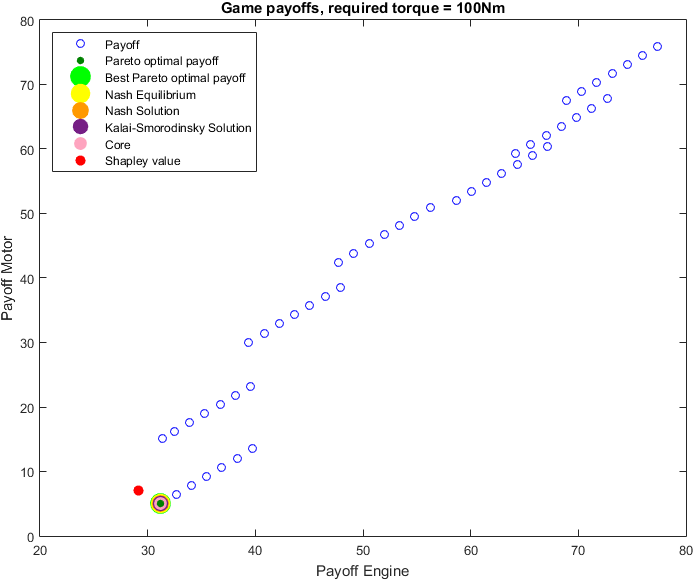
\includegraphics[scale=0.55]{figures/gametheory/100nm}
	\caption{Solutions for 100 Nm}
	\label{fig:100nm}
\end{figure}

\begin{figure}[h]
	\centering
	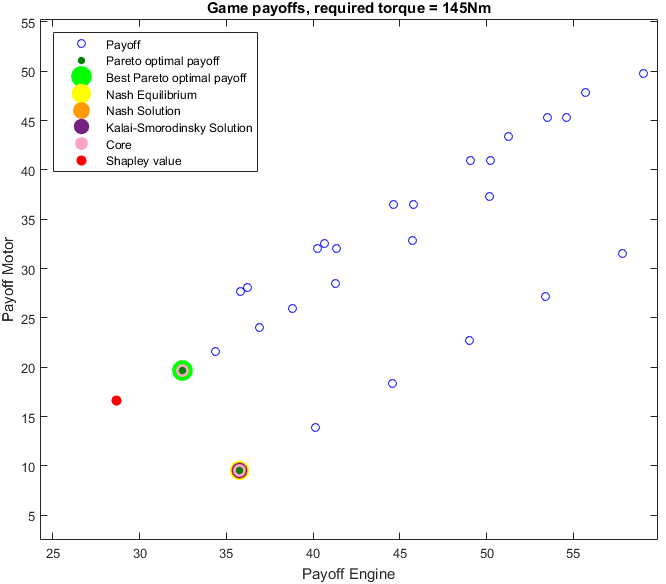
\includegraphics[scale=0.59]{figures/gametheory/145nm}
  	\caption{Solutions for 145 Nm}
  	\label{fig:145nm}
\end{figure}


For a torque demand of 178 \textit{Nm} Figure \ref{fig:178nm} shows that there are four different Pareto outcomes. All of them are also in the core. The best Pareto outcome is the left-most one and all of the other solutions Nash Equilibrium, Nash and Kalai-Smorodinsky solutions are equivalent with the right-most Pareto outcome. In the last Figure \ref{fig:280nm} with torque 280 \textit{Nm} there are again two Pareto outcomes.

\begin{figure}[h]
 	\centering
	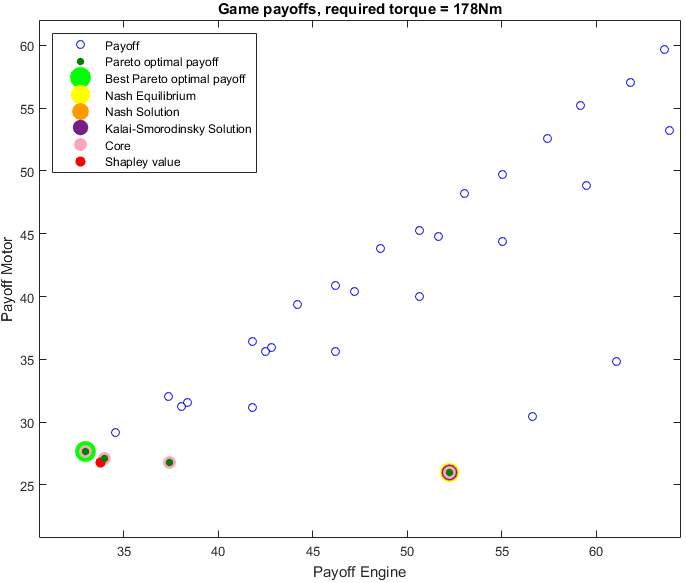
\includegraphics[scale=0.57]{figures/gametheory/178nm}
	\caption{Solutions for 178 Nm}
	\label{fig:178nm}
\end{figure}

\begin{figure}[h]
  	\centering
	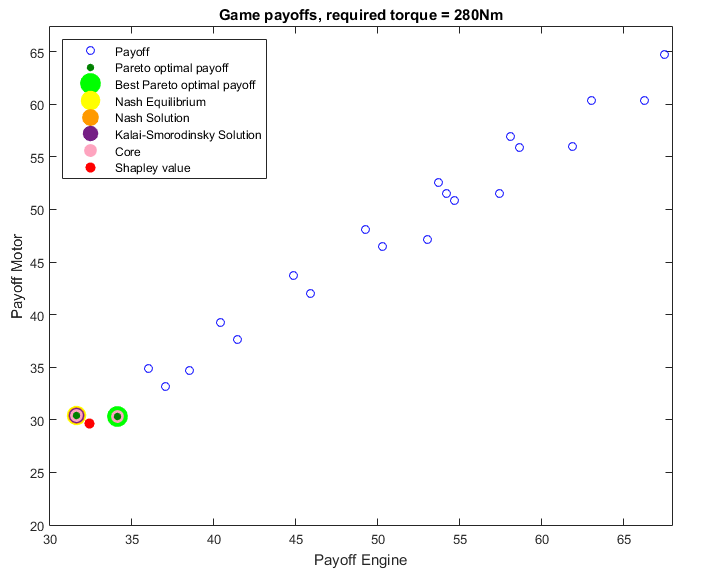
\includegraphics[scale=0.59]{figures/gametheory/280nm}
  	\caption{Solutions for 280 Nm}
  	\label{fig:280nm}
\end{figure}

\section{Hybrid Model Game-theoretical Simulation}

For each of the six game-theoretical solutions different scopes are presented, from which the most important one is the Game Theory scope, displaying the distribution of motor and engine torque. Then, the Drive Cycle and the Power Controller scopes are next in order of significance, because the Driver Cycle scope shows how the driver demands are met, which is the first goal of this game. The Power Controller is essential, because it displays the SOC of the battery along with the revolution speeds of the engine, motor and generator. Moreover, the Fuel and Emissions scope is crucial, since it concerns the second goal of the game - fuel consumption and gas emissions minimization. The Engine and Motor scopes show revolution speed, torque and power. For the first solution approach, the important scopes are given for the 5 phases of FTP75 and for the next five solution approaches only the Game Theory scope is shown, because little change can be noticed in the other scopes, while varying the choice of game-theoretical solution approach.

\subsection{Pareto Optimality}
This section deals with the first game-theoretical solution, Pareto Optimality, and its corresponding results during the FTP75 drive cycle. 

For FTP75-1 the results are displayed in Figures \ref{fig:gtpo1}, \ref{fig:dcpo1}, \ref{fig:pcpo1}, \ref{fig:fepo1}, \ref{fig:epo1} and \ref{fig:mpo1}. The pink line in Figure \ref{fig:dcpo1} is the demanded speed and the yellow is the actual speed. As it can be seen from Figure \ref{fig:gtpo1} the torque demand is distributed between the motor and engine. The engine can provide torque only in the range between 83-136 \textit{Nm} or 0 \textit{Nm}. In the other cases between -400 and 400 \textit{Nm} the motor can contribute without any limits. When the engine starts to contribute torque, the motor torque is decreased or it becomes 0. When the torque demand is higher than 136, then both the motor and the engine contribute to the powertrain with torque. At time 275-330s the torque demand rises to the maximum 400 \textit{Nm} because the battery SOC falls below 40 \% as seen in Figure \ref{fig:pcpo1}. At the same time the difference between demanded and actual speed grows up to a maximum of 70 \textit{km/h}; hence, the acceleration reaches its maximum of 1. The maximum speed of the drive cycle is reached at 240s and this is 91.25 \textit{km/h}. 

It should be noted that during the first simulation of the Pareto Optimality solution, a problem was encountered. At time 230-270s the engine revolution speed jumps up and down rapidly in a range from 2800-3300 \textit{rpm} or 293-345 \textit{rad/s}. Therefore, a hysteresis was implemented in this range in order to keep the revolution speed either at 2800 or at 3300 instead of letting it jitter. Nevertheless, the results are still not completely satisfactory, since the engine torque and power as in Figure \ref{fig:epo1} go up and down very quickly, although the revolution speed is restricted as much as possible. For the same reason the emissions and the fuel consumption are also unstable in the same time region in Figure \ref{fig:fepo1}.

\begin{figure}[hp]
\centering
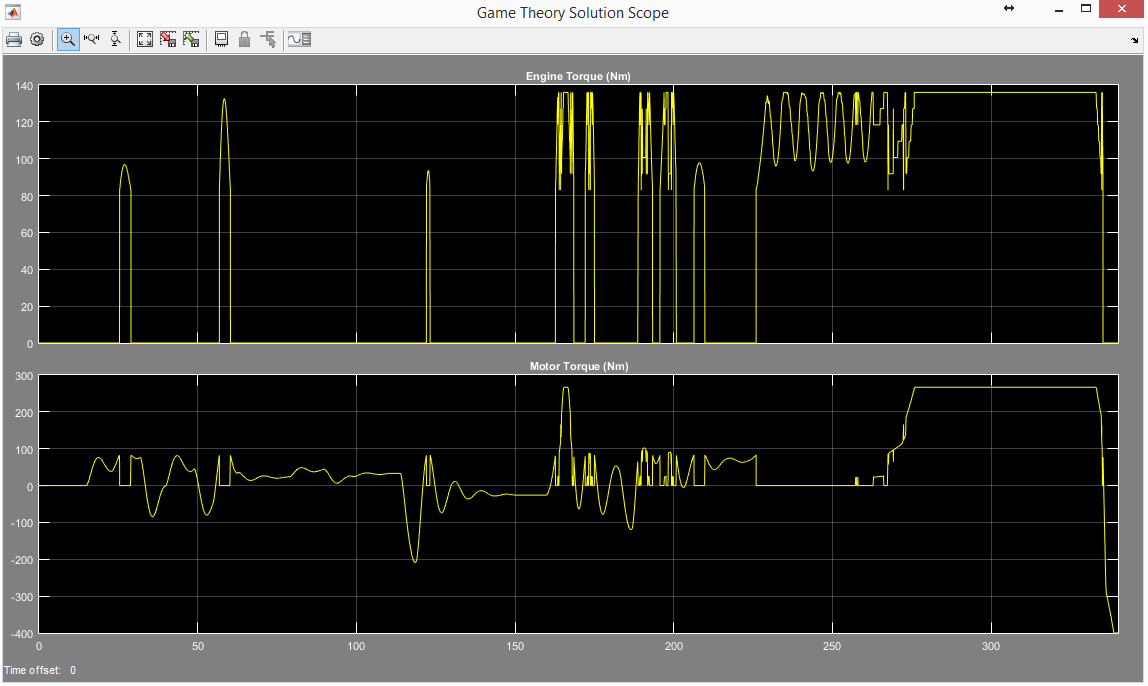
\includegraphics[scale=0.475]{figures/Pareto/FTP75-1/gameTheory30Juni}
\caption{Game Theory Scope With Pareto Optimality During FTP75-1}
\label{fig:gtpo1}
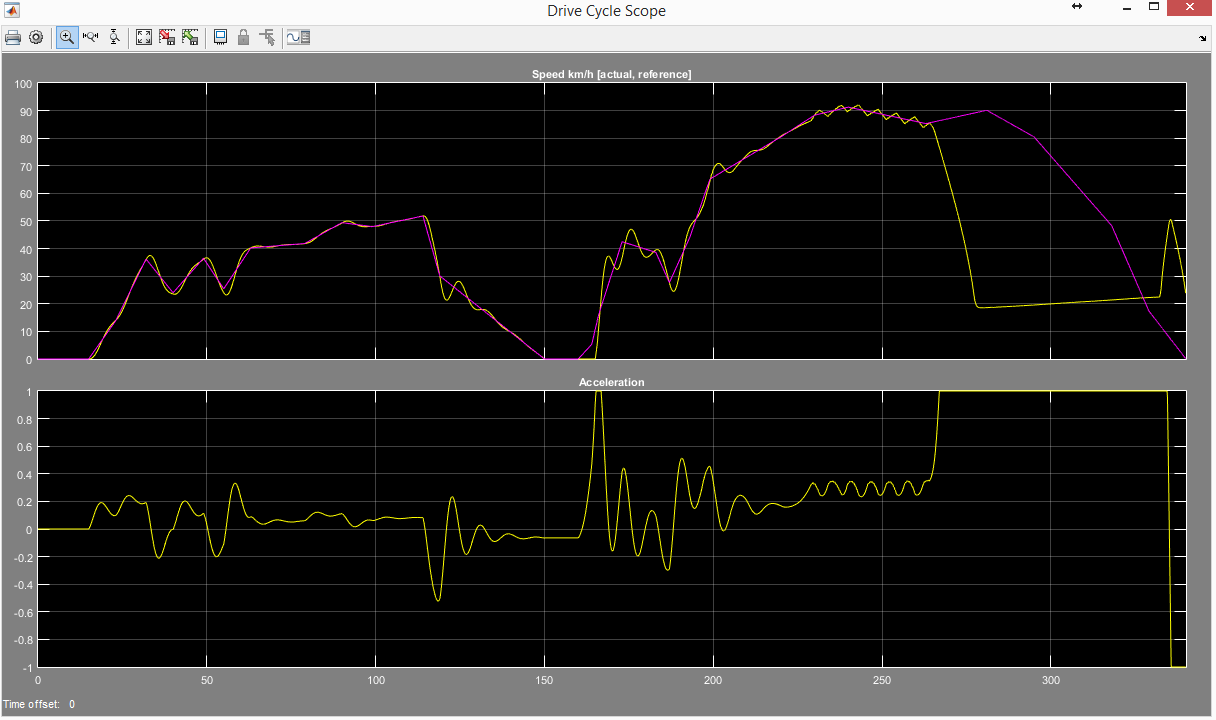
\includegraphics[scale=0.45]{figures/Pareto/FTP75-1/driveCycle30Juni}
\caption{Drive Cycle Scope With Pareto Optimality During FTP75-1}
\label{fig:dcpo1}
\end{figure}


\begin{figure}[hp]
\centering
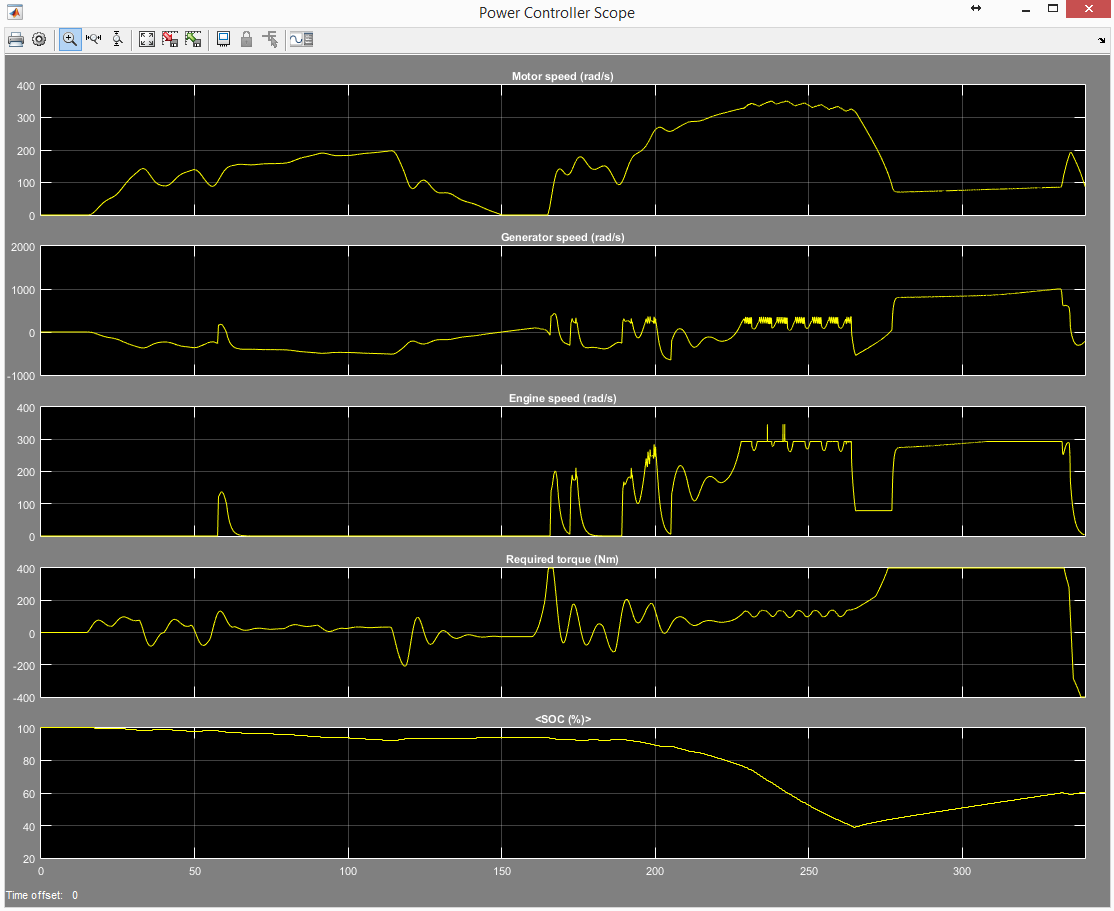
\includegraphics[scale=0.45]{figures/Pareto/FTP75-1/powerController30Juni}
\caption{Power Controller Scope With Pareto Optimality During FTP75-1}
\label{fig:pcpo1}
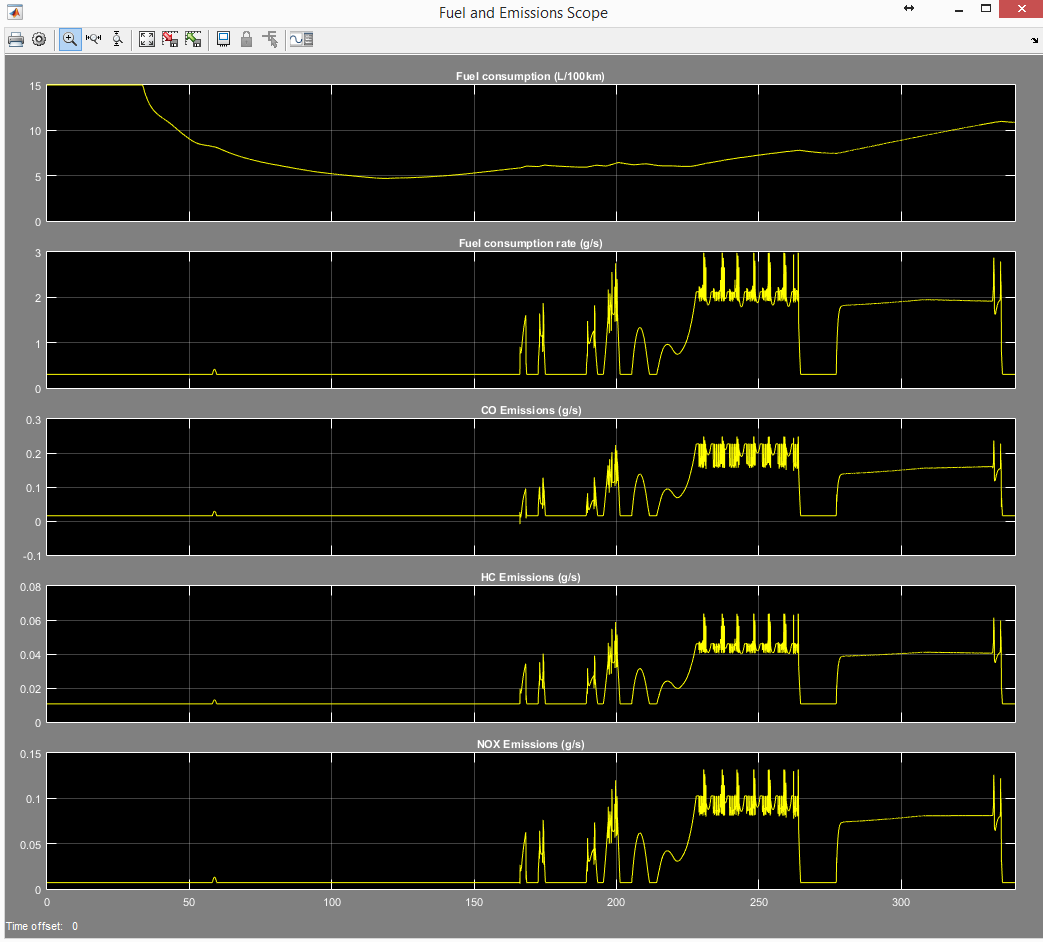
\includegraphics[scale=0.48]{figures/Pareto/FTP75-1/fuelEmissions30Juni}
\caption{Fuel And Emissions Scope With Pareto Optimality During FTP75-1}
\label{fig:fepo1}
\end{figure}


\begin{figure}[hp]
\centering
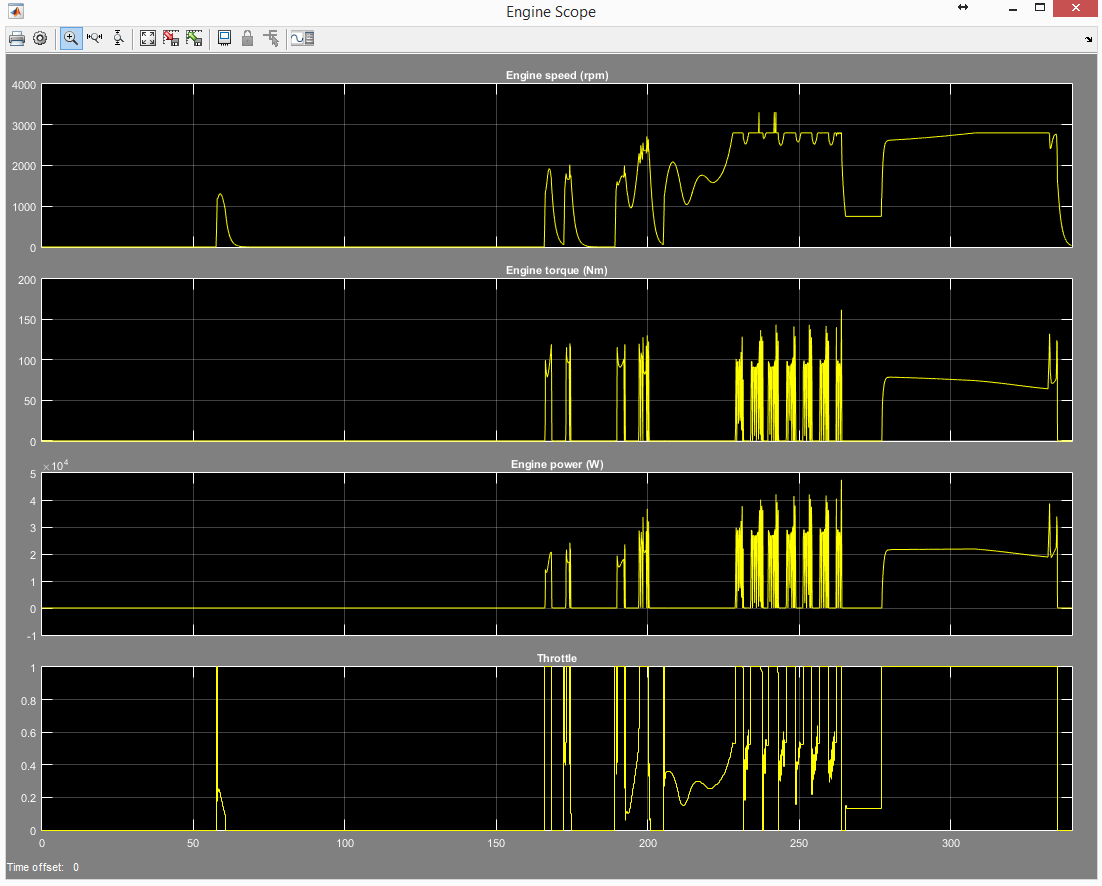
\includegraphics[scale=0.46]{figures/Pareto/FTP75-1/engine30Juni}
\caption{Engine Scope With Pareto Optimality During FTP75-1}
\label{fig:epo1}
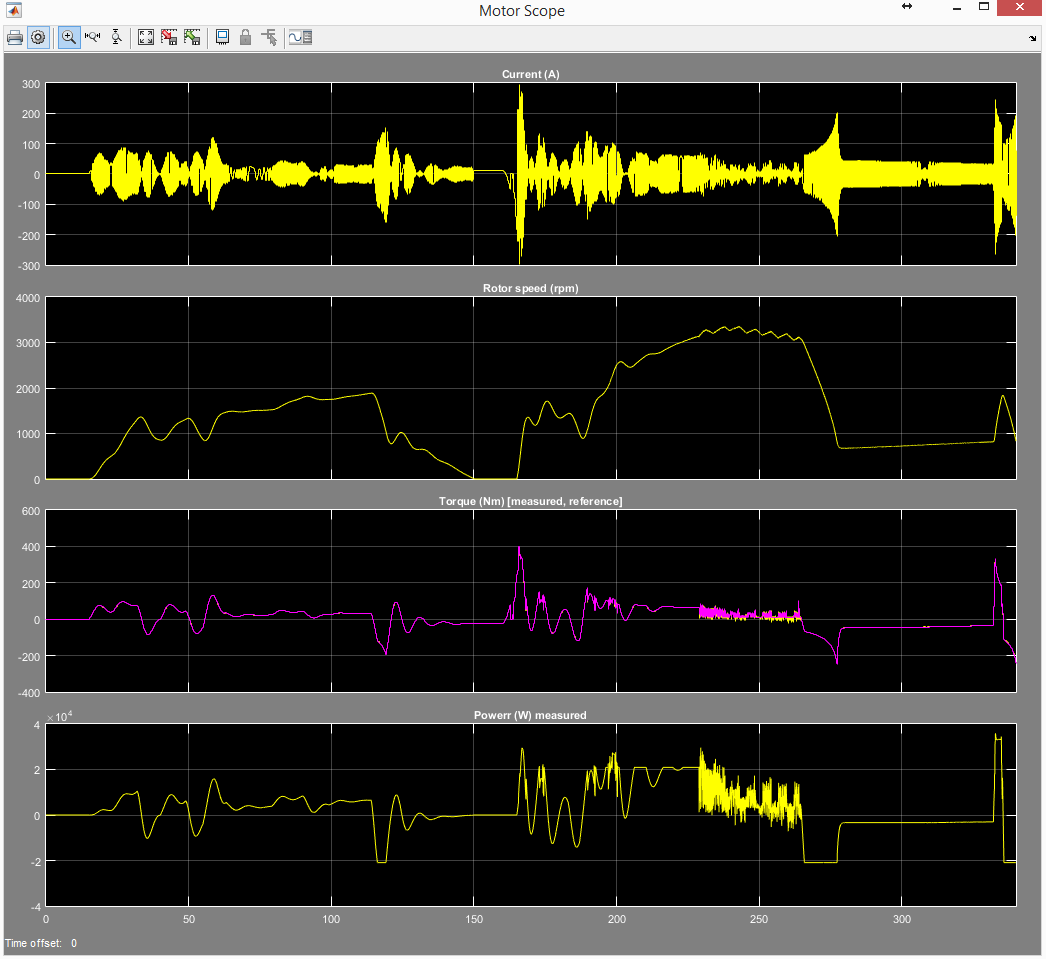
\includegraphics[scale=0.49]{figures/Pareto/FTP75-1/motor30Juni}
\caption{Motor Scope With Pareto Optimality During FTP75-1}
\label{fig:mpo1}
\end{figure}

The FTP75-2 results are in Figures \ref{fig:gtpo2}, \ref{fig:dcpo2}, \ref{fig:pcpo2}, \ref{fig:fepo2}, \ref{fig:epo2} and \ref{fig:mpo2}. In the second phase of the drive cycle there is a much frequent switching on and off of the engine compared to the first phase. Moreover, the motor requests negative torque much more often. This is due to the fact that in Figure \ref{fig:dcpo2} there are more decelerations than in Figure \ref{fig:dcpo1} where the braking power is automatically used for recharging. Since the battery SOC does not fall below 40 \% and it does not have to be recharged purposefully in FTP75-2, the drive cycle demands are met very well and the actual and demanded speed are always close. Therefore, this phase also runs very fast compared to FTP75-1.

\begin{figure}[hp]
\centering
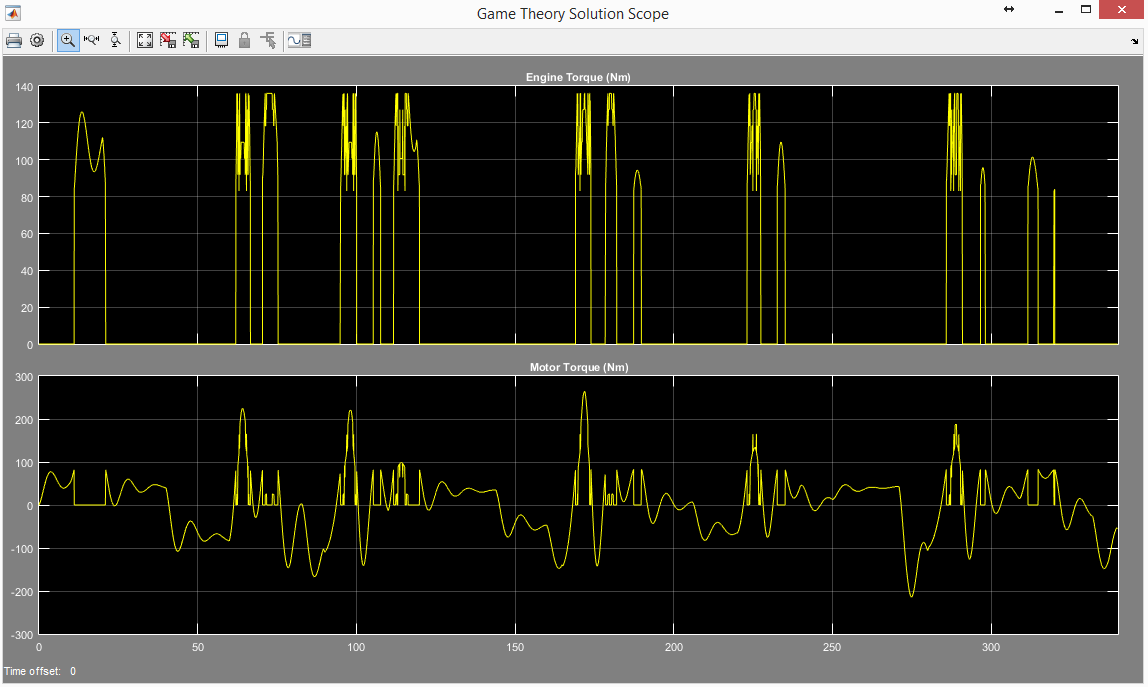
\includegraphics[scale=0.46]{figures/Pareto/FTP75-2/gameTheory03Juli}
\caption{Game Theory Scope With Pareto Optimality During FTP75-2}
\label{fig:gtpo2}
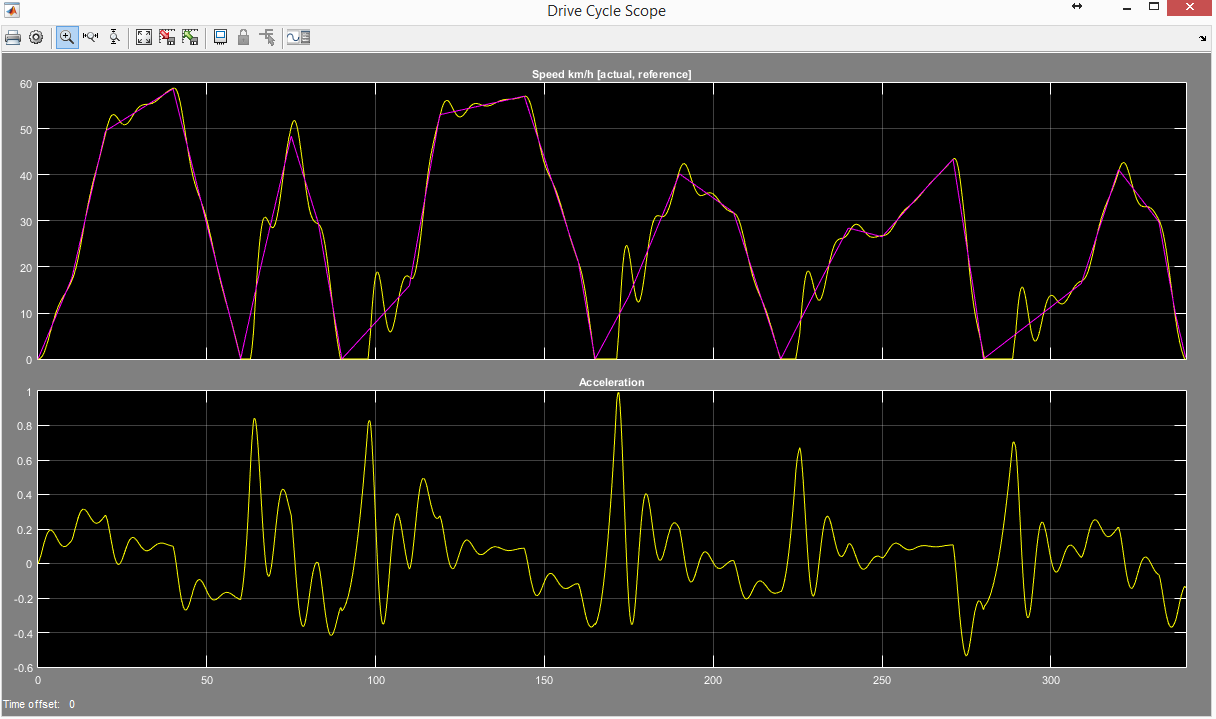
\includegraphics[scale=0.44]{figures/Pareto/FTP75-2/driveCycle03Juli}
\caption{Drive Cycle Scope With Pareto Optimality During FTP75-2}
\label{fig:dcpo2}
\end{figure}

\begin{figure}[hp]
\centering
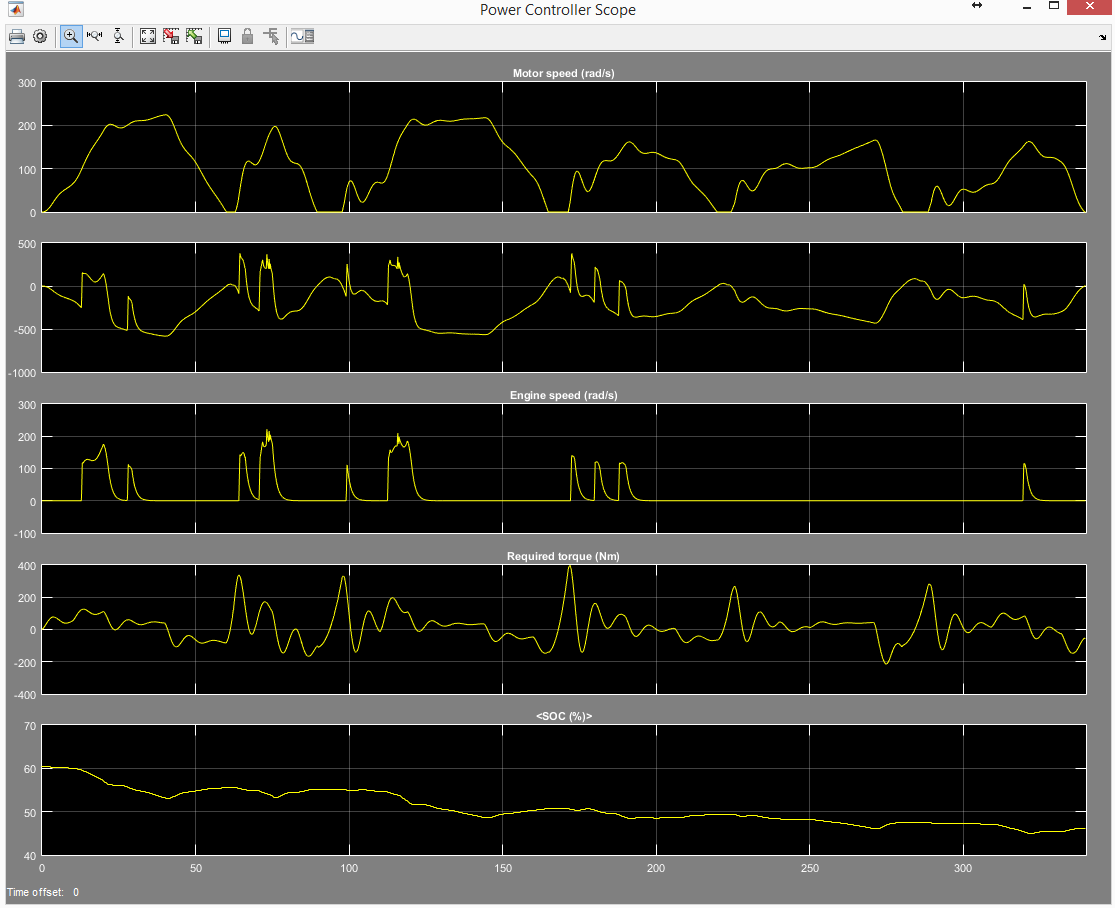
\includegraphics[scale=0.44]{figures/Pareto/FTP75-2/powerController03Juli}
\caption{Power Controller Scope With Pareto Optimality During FTP75-2}
\label{fig:pcpo2}
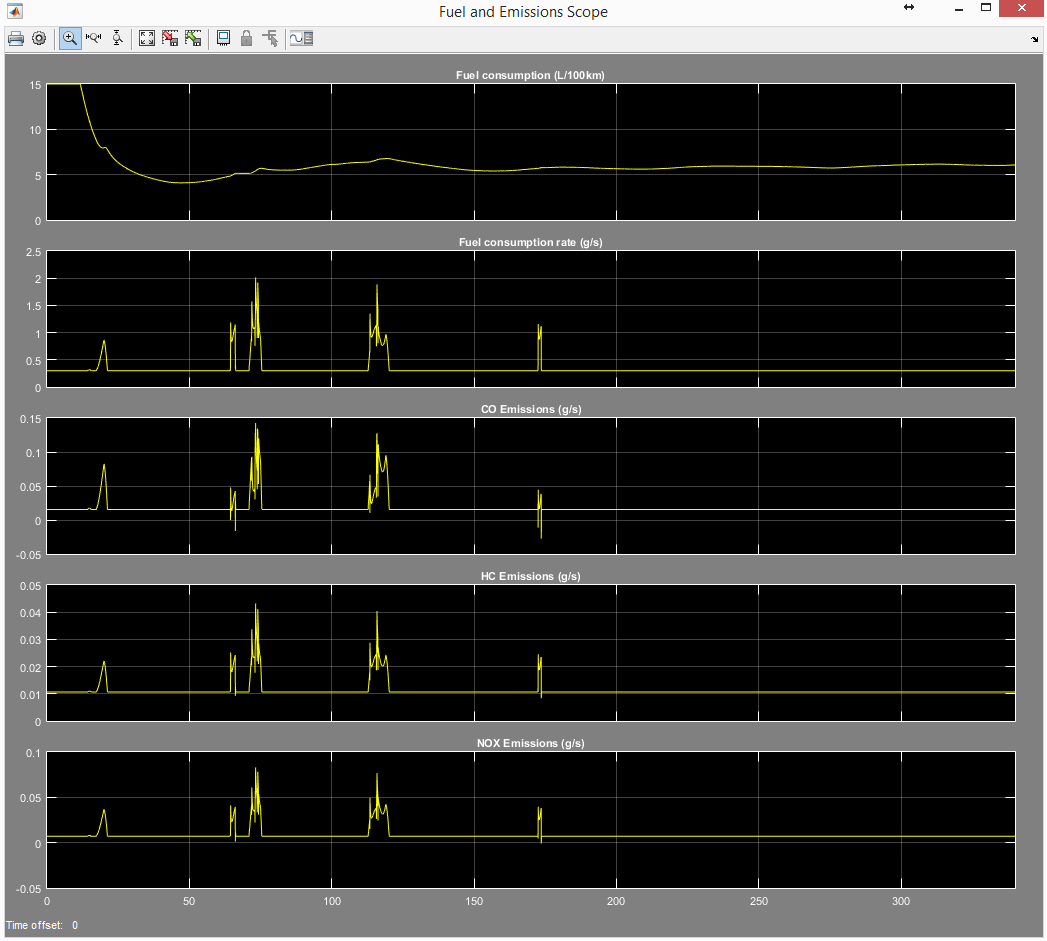
\includegraphics[scale=0.47]{figures/Pareto/FTP75-2/fuelEmissions03Juli}
\caption{Fuel and Emissions Scope With Pareto Optimality During FTP75-2}
\label{fig:fepo2}
\end{figure}

\begin{figure}[hp]
\centering
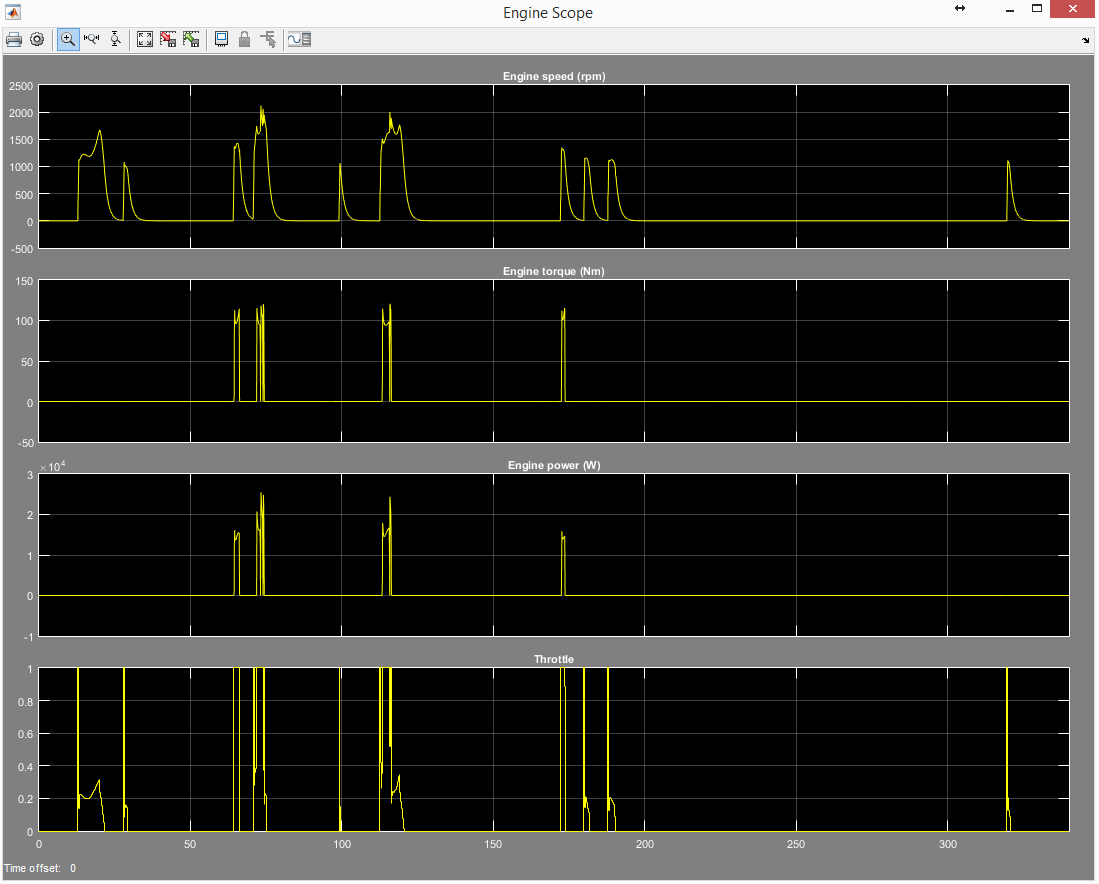
\includegraphics[scale=0.45]{figures/Pareto/FTP75-2/engine03Juli}
\caption{Engine Scope With Pareto Optimality During FTP75-2}
\label{fig:epo2}
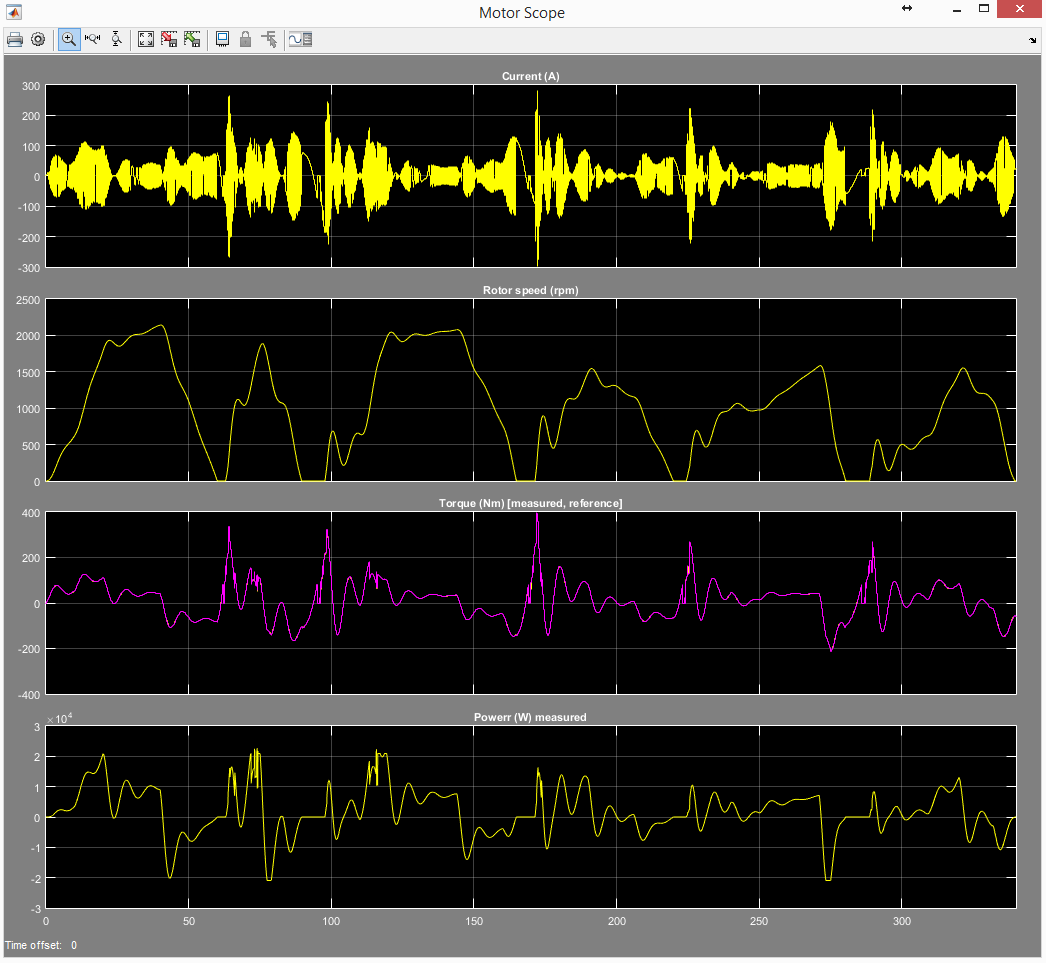
\includegraphics[scale=0.48]{figures/Pareto/FTP75-2/motor03Juli}
\caption{Motor Scope With Pareto Optimality During FTP75-2}
\label{fig:mpo2}
\end{figure}

In FTP75-3 as shown in Figures \ref{fig:gtpo3}, \ref{fig:dcpo3}, \ref{fig:pcpo3} and \ref{fig:epo3} the SOC again falls below 40 \% and then the difference between actual and demanded speed becomes at most 25 \textit{km/h}. This happens at time 120s and thus the acceleration is increased to the maximum of 1 and the required torque becomes 400 \textit{Nm}. During this time the engine and the motor are both prompted for torque constantly. When the battery is recharged to 60 \% at 180s, the actual speed still undergoes a lot of changes until it meets the required speed at time 250s. The reason is that the acceleration has been constantly 1 for a very long and then it suddenly drops to -1. The motor, engine and generator revolution speeds are also kept constant during recharge mode. Furthermore, in Figure \ref{fig:epo3} it can be seen that the problem with the rapid change of torque from the engine does not occur because there is no jittering of the engine revolution speed or torque.

\begin{figure}[hp]
\centering
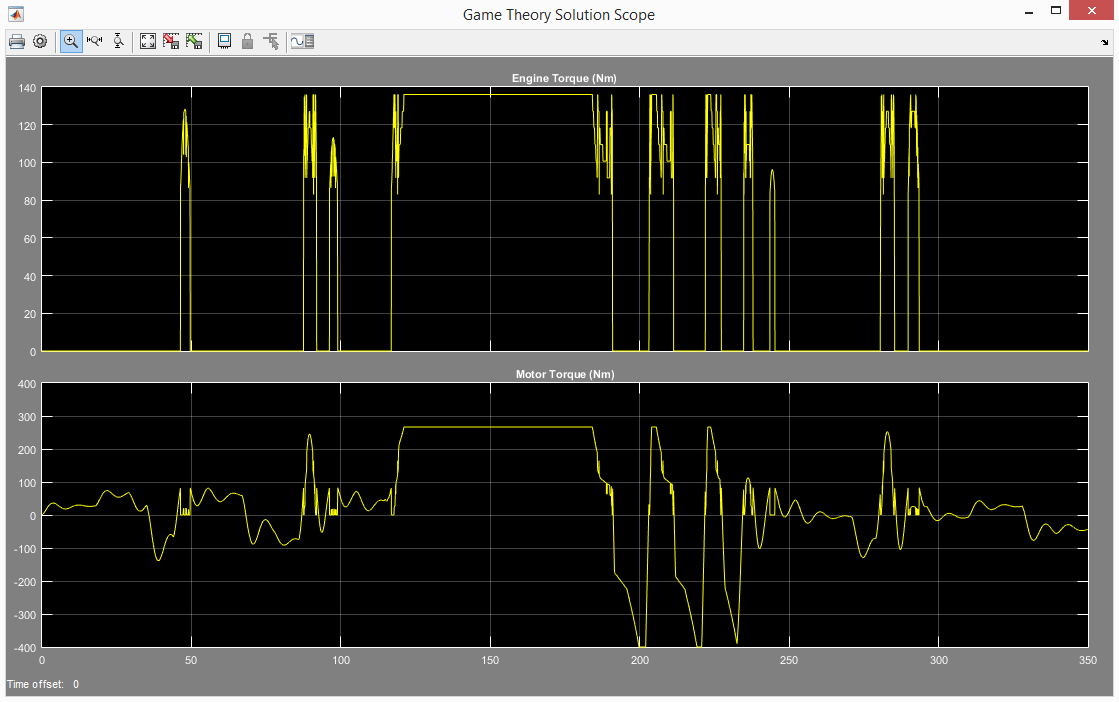
\includegraphics[scale=0.48]{figures/Pareto/FTP75-3/gameTheory08Juni}
\caption{Game Theory Scope With Pareto Optimality During FTP75-3}
\label{fig:gtpo3}
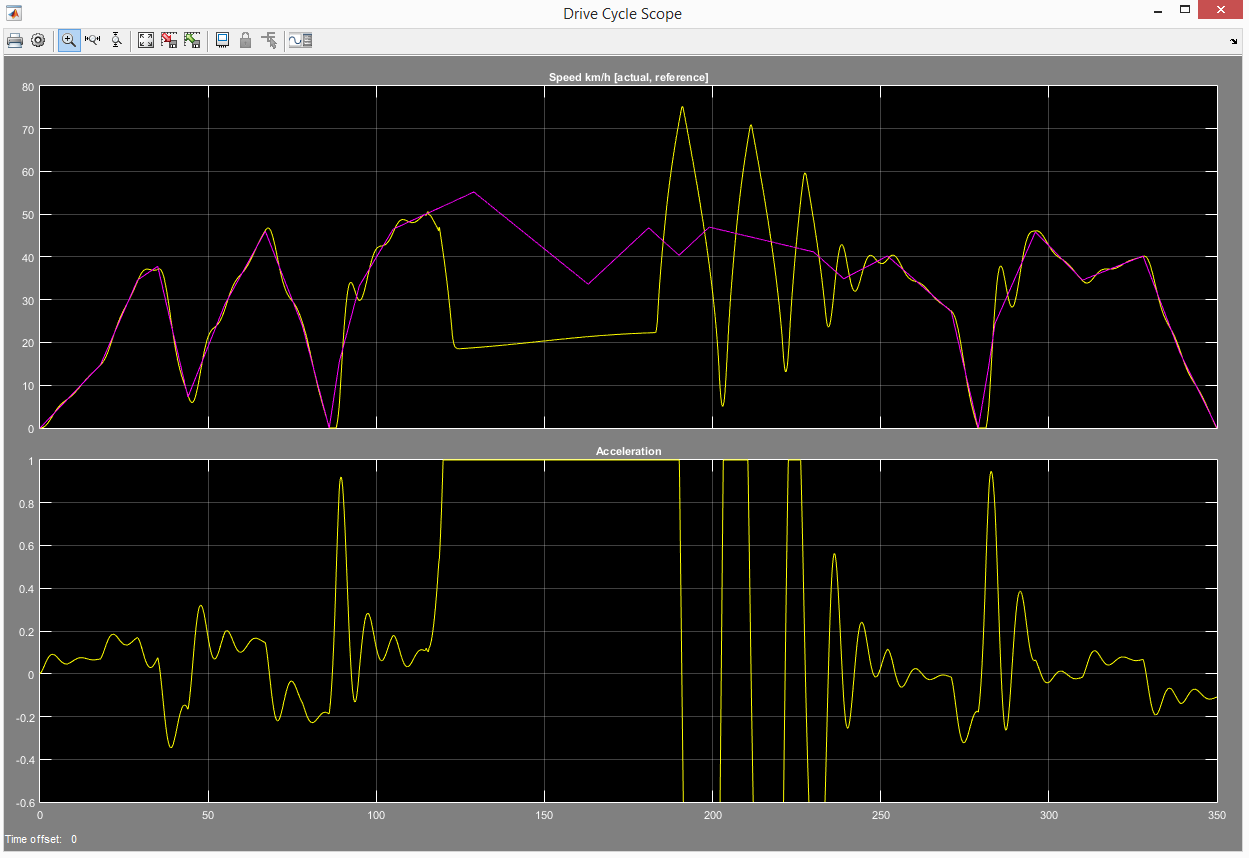
\includegraphics[scale=0.43]{figures/Pareto/FTP75-3/driveCycle08Juni}
\caption{Drive Cycle Scope With Pareto Optimality During FTP75-3}
\label{fig:dcpo3}
\end{figure}

\begin{figure}[hp]
\centering
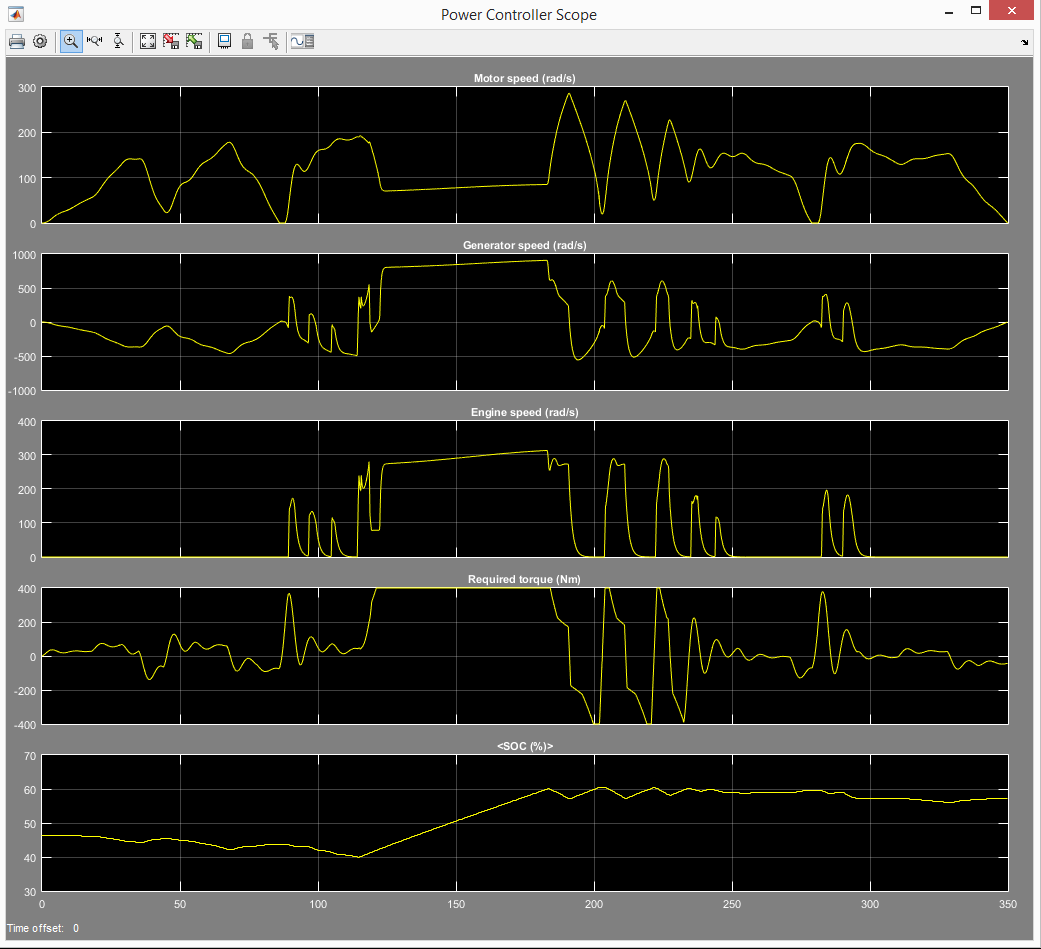
\includegraphics[scale=0.47]{figures/Pareto/FTP75-3/powerController08Juni}
\caption{Power Controller Scope With Pareto Optimality During FTP75-3}
\label{fig:pcpo3}
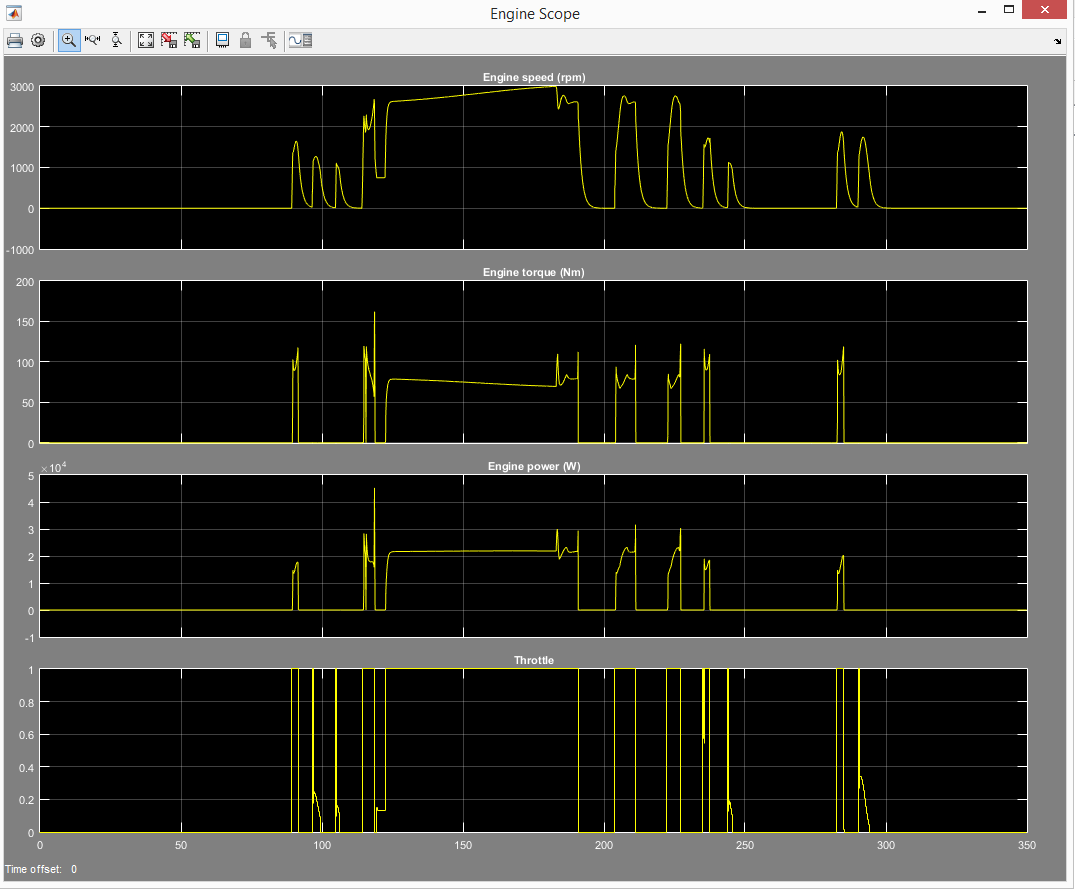
\includegraphics[scale=0.46]{figures/Pareto/FTP75-3/engine08Juni}
\caption{Engine Scope With Pareto Optimality During FTP75-3}
\label{fig:epo3}
\end{figure}


In FTP75-4 results are displayed in Figure \ref{fig:gtpo4}, \ref{fig:dcpo4}, \ref{fig:pcpo4} and \ref{fig:mpo4}. Similarly to the FTP75-2, in FTP75-4 the motor is prompted for negative torque much more frequently than the other phases, because there are more sudden accelerations and decelerations and the speed demand is changing more abruptly. It can be concluded that in this phase the drive cycle demands are again met very accurately like in FTP75-2 as in \ref{fig:dcpo4}. The battery mode in Figure \ref{fig:pcpo4} keeps alternating from recharge mode during deceleration with negative torque and discharge mode during acceleration with positive torque.

\begin{figure}[hp]
\centering
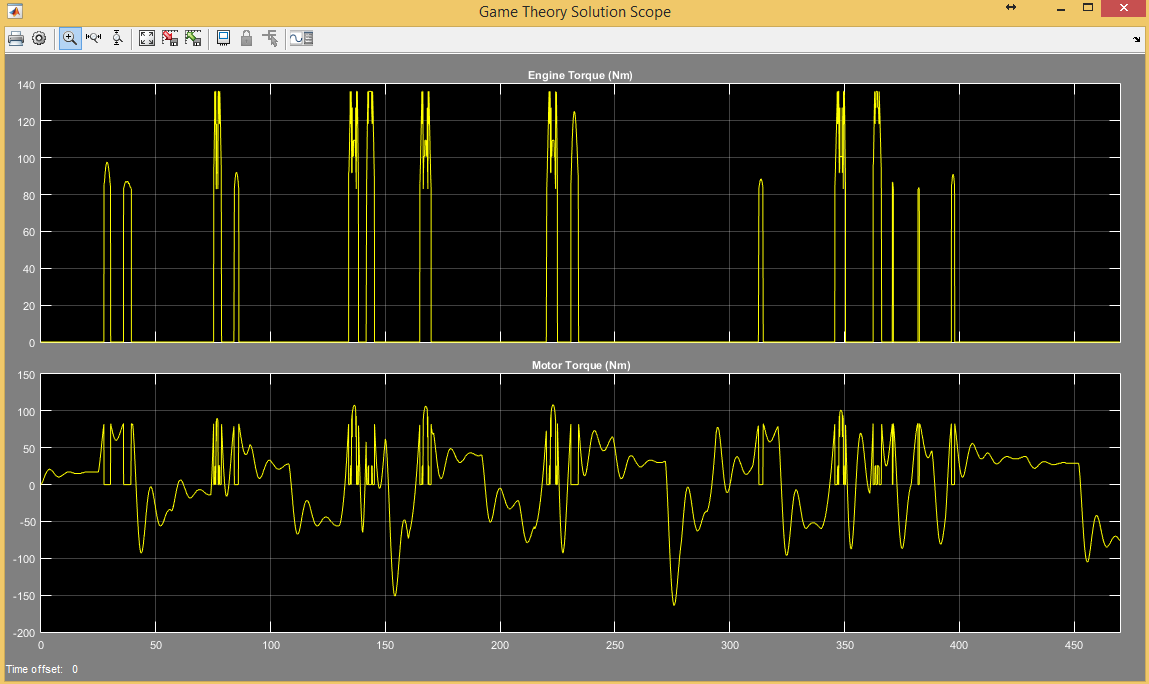
\includegraphics[scale=0.46]{figures/Pareto/FTP75-4/gameTheory05Juli}
\caption{Game Theory Scope With Pareto Optimality During FTP75-4}
\label{fig:gtpo4}
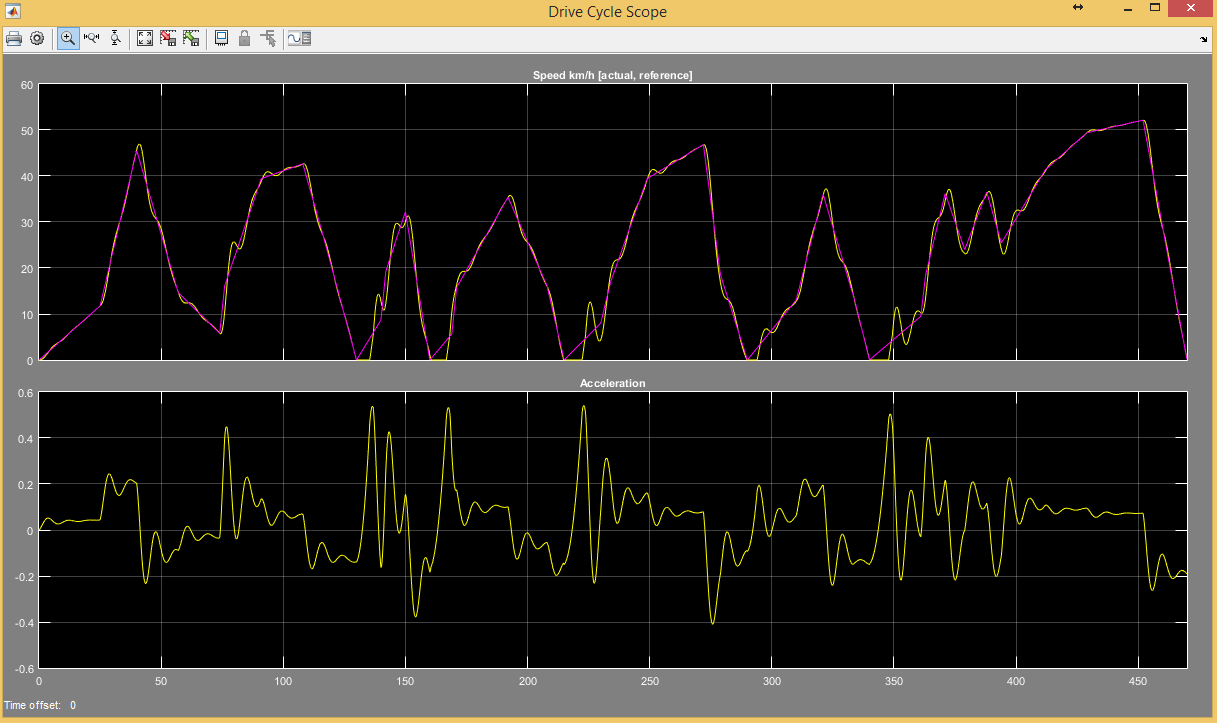
\includegraphics[scale=0.44]{figures/Pareto/FTP75-4/driveCycle05Juli}
\caption{Drive Cycle Scope With Pareto Optimality During FTP75-4}
\label{fig:dcpo4}
\end{figure}

\begin{figure}[hp]
\centering
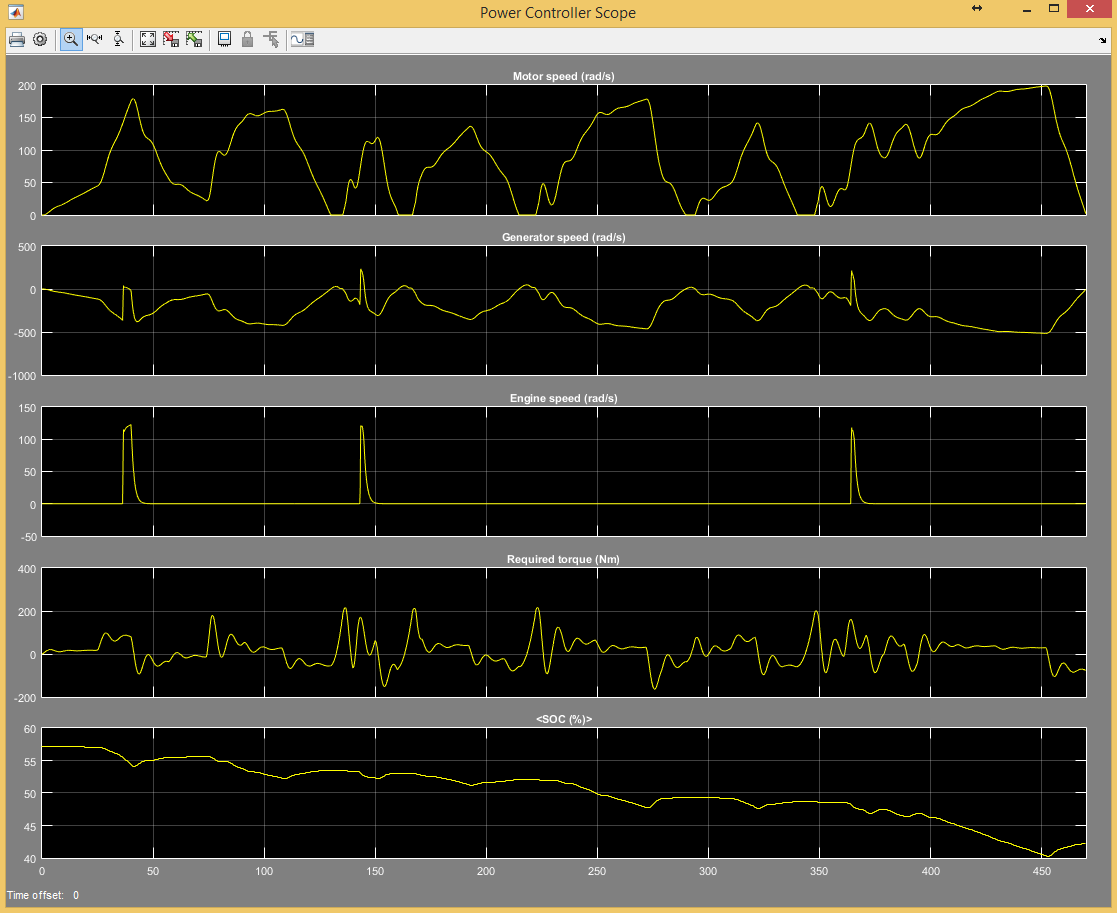
\includegraphics[scale=0.45]{figures/Pareto/FTP75-4/powerController05Juli}
\caption{Power Controller Scope With Pareto Optimality During FTP75-4}
\label{fig:pcpo4}
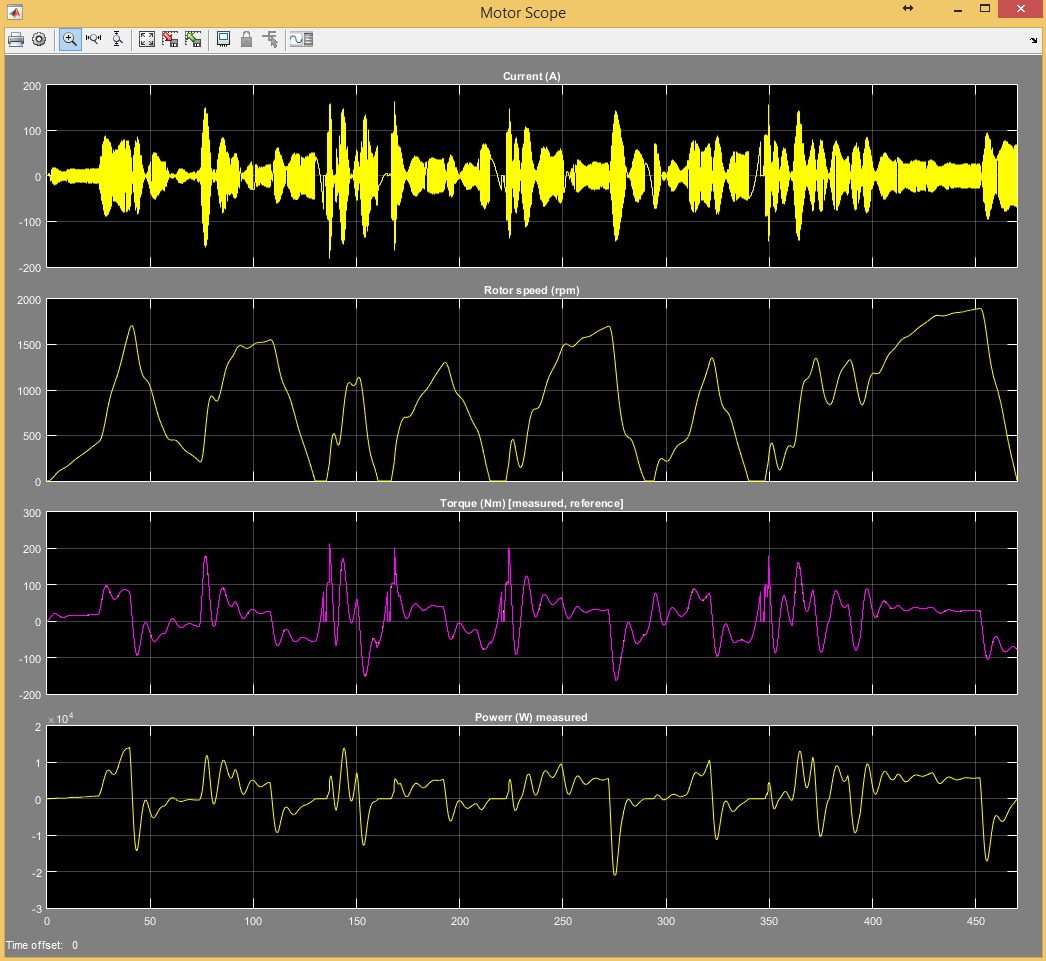
\includegraphics[scale=0.48]{figures/Pareto/FTP75-4/motor05Juli}
\caption{Motor Scope With Pareto Optimality During FTP75-4}
\label{fig:mpo4}
\end{figure}

In the last phase FTP75-5 in Figures \ref{fig:gtpo5}, \ref{fig:dcpo5}, \ref{fig:pcpo5} and \ref{fig:mpo5}, the battery has to be recharged at 50s and the maximum difference of demanded and actual speed this incurs is 70 \textit{km/h}. During recharge mode the engine and motor are constantly contributing torque, because the torque demand is high. At 110s the maximum speed of this phase 91.25 \textit{km/h} is reached. At 120s the battery is already at the target 60 \% and the actual speed tries to keep up with the demanded speed. However, it goes up and down before it comes to the right demanded speed at 170s, similarly as in FTP75-3. After acceleration was kept constant, it takes time for it to adjust to the right amount and influence the actual speed correctly. After 170s the actual speed starts to meet the demand again. 

For the next game-theoretical approaches only the Game Theory scope will be shown, since there is little difference in the other scopes. Moreover, it is crucial to examine the motor and engine torque distribution differences between the different game theory approaches because that is the main topic in this thesis.

\begin{figure}[hp]
\centering
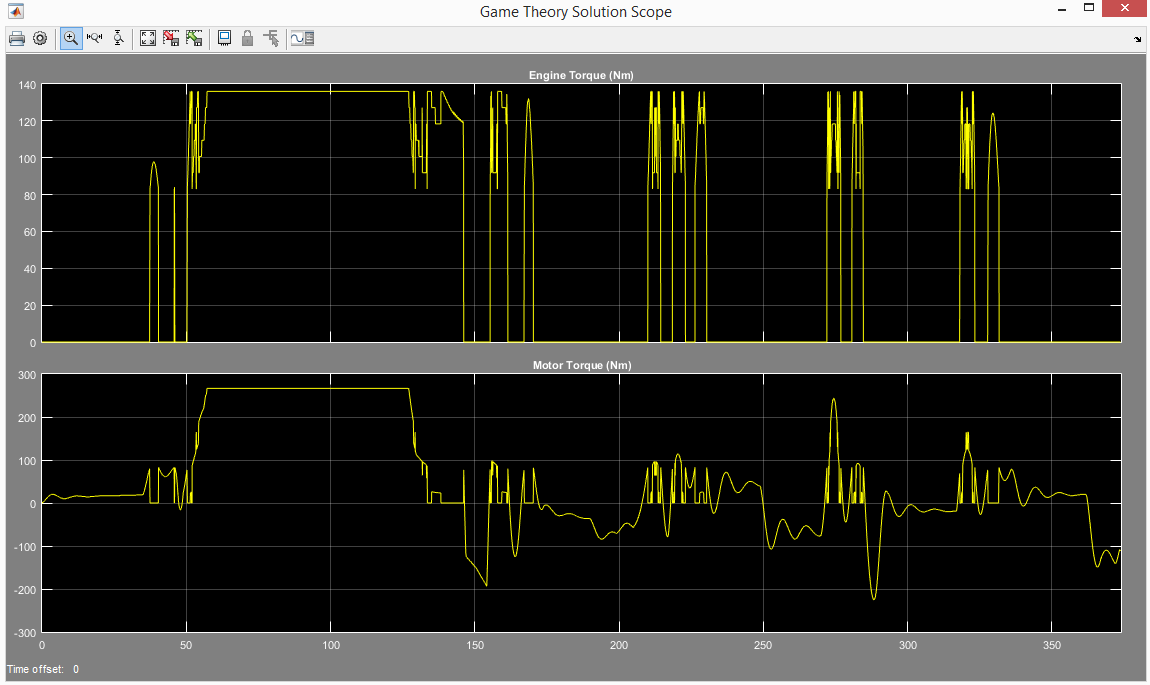
\includegraphics[scale=0.46]{figures/Pareto/FTP75-5/gameTheory05Juli}
\caption{Game Theory Scope With Pareto Optimality During FTP75-5}
\label{fig:gtpo5}
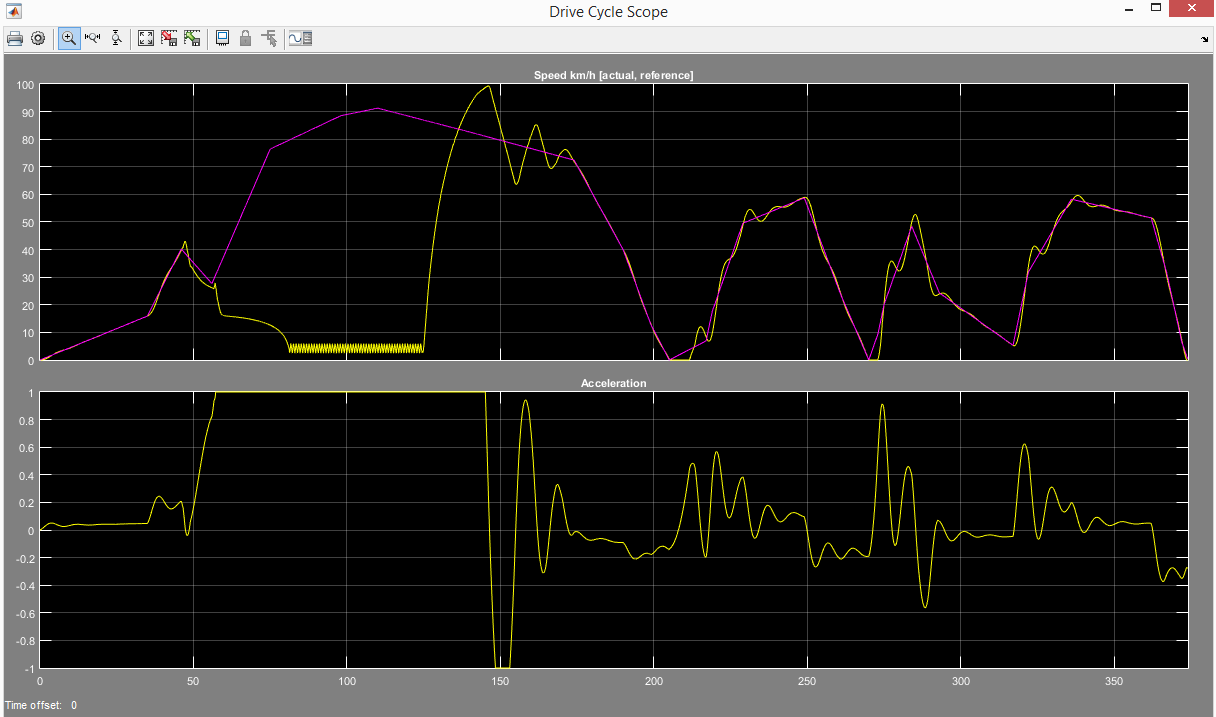
\includegraphics[scale=0.44]{figures/Pareto/FTP75-5/driveCycle05Juli}
\caption{Drive Cycle Scope With Pareto Optimality During FTP75-5}
\label{fig:dcpo5}
\end{figure}

\begin{figure}[hp]
\centering
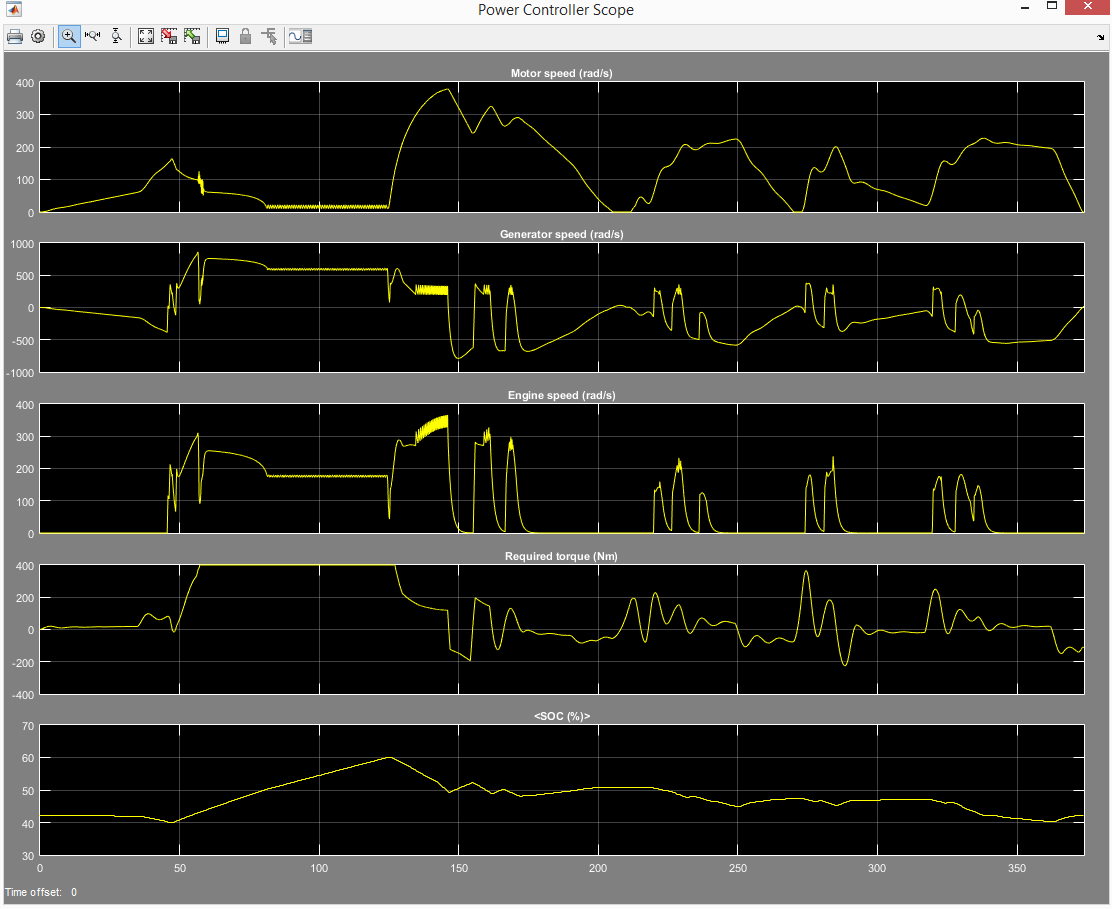
\includegraphics[scale=0.46]{figures/Pareto/FTP75-5/powerController05Juli}
\caption{Power Controller Scope With Pareto Optimality During FTP75-5}
\label{fig:pcpo5}
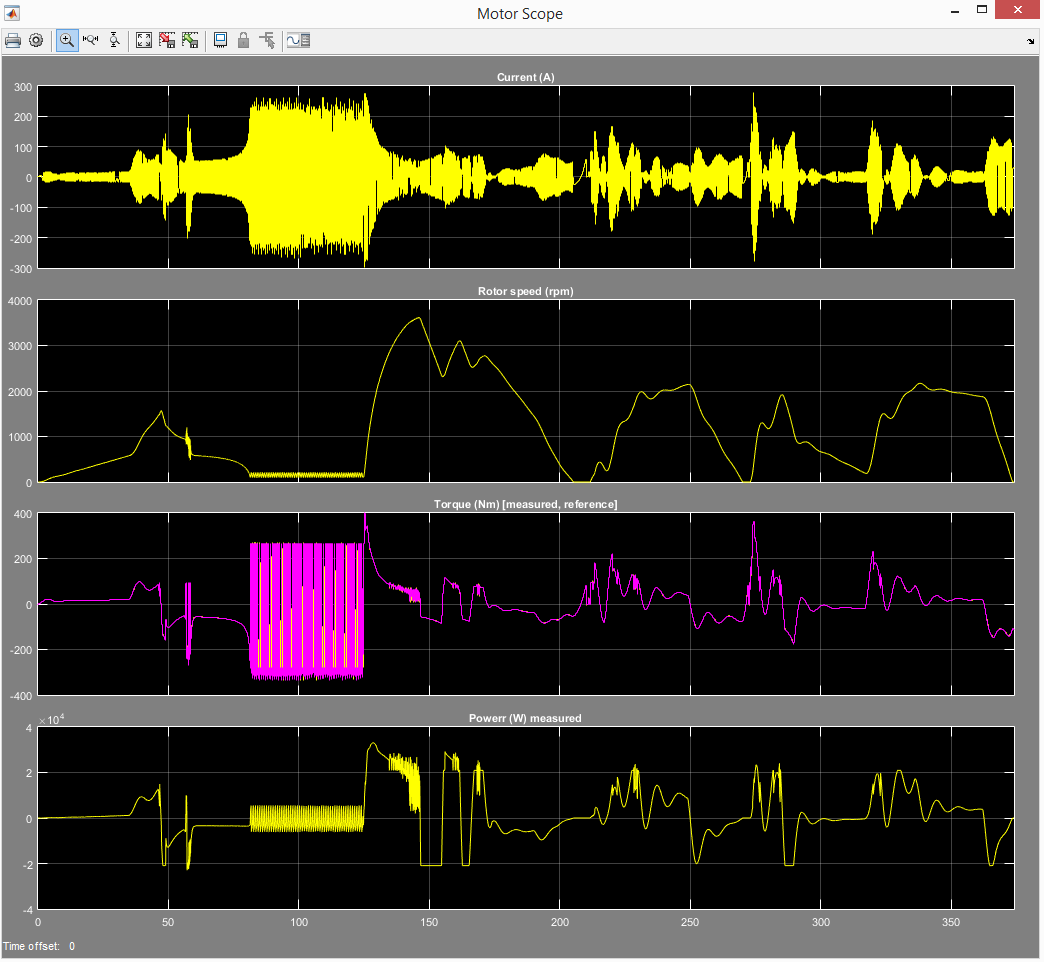
\includegraphics[scale=0.48]{figures/Pareto/FTP75-5/motor05Juli}
\caption{Motor Scope With Pareto Optimality During FTP75-5}
\label{fig:mpo5}
\end{figure}

\subsection{Nash Equilibrium}
This section discusses the Game Theory scope of all of the five phases in the FTP75 drive cycle when the game is solved with Nash Equilibrium. The results are compared to the Pareto Optimality solution. FTP75-1, FTP75-2, FTP75-3, FTP75-4 and FTP75-5 results are displayed respectively in Figures \ref{fig:gtne1}, \ref{fig:gtne2}, \ref{fig:gtne3}, \ref{fig:gtne4} and \ref{fig:gtne5} in Appendix \ref{app:1}.

As seen in Figure \ref{fig:gtne1} FTP75-1 of the Nash Equilibrium produces slight differences in comparison with Figure \ref{fig:gtpo1}. In particular, the engine torque demand at time 160-165s is wider with Nash Equilibrium than with Pareto Optimality. In the former solution it ranges between 110-136 \textit{Nm} and in the latter its range is between 85-136 \textit{Nm}. Then at time 170-175s with Nash Equilibrium solution the engine torque demand goes directly from 0 to 136 and back to 0 \textit{Nm} again, whereas with Pareto Optimality it jumps between 85 and 136 \textit{Nm}. At time 230-270s the Nash Equilibrium again performs better, because the engine torque, which looks sinusoidal, undergoes less changes than with Pareto Optimality. The same conclusions at the same time periods are drawn also for the motor torque, whose change depends on the engine torque.

Similarly, for all of the remaining phases FTP75-2, FTP75-3, FTP75-4 and FTP75-5 the Nash Equilibrium also produces more stable engine torque solutions than Pareto Optimality.

\subsection{Nash Bargaining Solution}
The Nash Bargaining solution presented in Figure \ref{fig:gtns1} results are very similar to the Nash Equilibrium in Figure \ref{fig:gtne1}. Therefore, the FTP75 results of the Nash Bargaining solution will be primarily compared to the Nash Equilibrium results. The similarity is due to the fact that the Nash Equilibrium output was used for computing the Nash Equilibrium because it was taken as the conflict point as described in subsection \ref{subsec:nashbargFun}.

Despite the similarity, in FTP75-1 there is a difference at time from 160s to 170s in Figure \ref{fig:gtne1} where the Nash Equilibrium requests the maximum engine torque of 136 \textit{Nm} and then requests 115 \textit{Nm}, whereas in the Nash Bargaining solution in Figure \ref{fig:gtns1} after prompting for 136 \textit{Nm} it goes down to 90 \textit{Nm}. The same happens between 190s and 200s. Furthermore, the next difference is visible between 230s and 275s, where the motor torque is 0 \textit{Nm} and the engine torque in Nash Equilibrium is changing in the range from 100 to 128 \textit{Nm}. In the Nash Bargaining solution this also happens, but the change is more abrupt and it is either 100 or 128 \textit{Nm} rather than taking values in between them. Except for these cases, the game theory solutions with Nash Equilibrium and with Nash Bargaining solution are the same.

FTP75-2, FTP75-3, FTP75-4 and FTP75-5 are also very similar to the Nash Equilibrium. The visible difference in all of them is that the Nash Bargaining solution requests a wider range of torque from the engine, from 95 to 136 \textit{Nm}, while the Nash Equilibrium requests from only 110 to 136 \textit{Nm}.

\subsection{Kalai-Smorodinsky Solution}
The Kalai-Smorodinsky solution produces exactly the same results as the Nash solution does for FTP75-1 and FTP75-2 as shown in Figures \ref{fig:gtks1}, \ref{fig:gtks2}. The first visible difference between the two solutions appears in FTP75-3 in Figure \ref{fig:gtks3} at time 235-240s where the Kalai-Smorodinsky solution of the motor torque is going up and down from 0 to 90 repeatedly \textit{Nm}, while the Nash solution repeats this only 2 times. This also affects the engine torque which behaves similarly in the range from 95 to 136 \textit{Nm} in the Kalai-Smorodinsky solution, but rather stays at 136 \textit{Nm} for the Nash solution. In FTP75-4 and FTP75-5 in Figures \ref{fig:gtks4} and \ref{fig:gtks5} there is no difference between the two solutions. The almost identical results of the Kalai-Smorodinsky and the Nash solution come from fact that their concepts are very similar. Firstly, they both use the conflict point as a part of the computation. The Kalai-Smorodinksy solution is assumed to be an extension of the Nash solution by taking into account additionally the ideal minimum payoff point.

\subsection{Core}
Solving the game with the Core generates exactly the same results as Pareto Optimality, due to the fact that all outcomes which are in the core are always Pareto optimal and in two-player cooperative games the two concepts produce equivalent solutions. Therefore, the Simulink scopes of the Core are not shown. However to prove that the core was also simulated, the fuel, emissions and battery related values are shown in the tables in the next section \ref{sec:goalresults}.

\subsection{Shapley Value}
After the implementation of the last game-theoretical solution as described in \ref{subsec:shapleyimpl}, the simulation was found to be extremely slow mainly because of the \textit{mixedstrategies.m} function, which contains the slow \textit{linprog} function. Without the \textit{linprog} function a coalitional form of the game for the individual coalitions $\{1\}$ and $\{2\}$ cannot be found; hence, the concept of Shapley value would not have been applicable at all. Taking into account the importance of \textit{linprog}, it is impossible to replace it with another faster function, because a system of linear equations has to be solved at any case. For this reason and also because of the large number of result scopes in the Appendices, it was decided that the Shapley Value will not be simulated.

\section{Fuel, Emissions And Battery}
\label{sec:goalresults}
The last section of this chapter describes the results, related to the second goal of the game - fuel consumption and gas emissions minimization and the battery SOC.

\subsection{Fuel Consumption And Gas Emissions}
To address the goal of fuel economy and minimizing gas emissions, the following results are presented in Table \ref{tab:fuelEmis}. After a thorough examination of total fuel, fuel consumption, CO, HC and NOX emissions, a few conclusions can be made. Firstly, the best results for total fuel are generated from the Nash Solution and the Kalai-Smorodinksy for FTP75 phases 1 to 4. Only in FTP75-5 the latter solution outperforms the former. However, in FTP75-5 Pareto Optimality achieves minimum fuel consumption of 10.79 \textit{g/s} and also minimum total fuel of 1.47 \textit{g/s}. With regard to gas emissions, all of the solutions have similar results and vary slightly, but from all drive cycle phases it can be deduced that the Pareto Optimality performs best in the most cases.

\begin{table}[h]
\centering
\begin{tabular}{ |p{1.5cm}|p{1.5cm}|p{1.3cm}|p{1.3cm}|p{1.3cm}|p{1.3cm}|p{1.3cm}|} 
 \hline
  \cline{3-7}
   & Drive cycle & \multicolumn{5}{|c|}{Game-theoretical solution} \\
   \cline{3-7}
   & & Pareto Optimality & Nash Equilibrium & Nash Solution & Kalai- Smorodinsky Solution & The Core \\
 \hline\hline
 \multirow{5}{*}{\parbox{1.5cm}{Total fuel (l)}} 
 & FTP75-1 & 0.398 & 0.406 & 0.397 & 0.397 & 0.398 \\ 
 & FTP75-2 & 0.554 & 0.5635 & 0.554 & 0.554 & 0.554 \\  
 & FTP75-3 & 0.917 & 0.901 & 0.893 & 0.893 & 0.895 \\ 
 & FTP75-4 & 1.112 & 1.097 & 1.089 & 1.09 & 1.091 \\ 
 & FTP75-5 & 1.47 & 1.566 & 1.543 & 1.513 & 1.46 \\ 
 \hline 
 \multirow{5}{*}{\parbox{1.5cm}{Fuel consumption (g/s)}} 
 & FTP75-1 & 10.88 & 11.13 & 10.85 & 10.85 & 10.88 \\ 
 & FTP75-2 & 6.077 & 6.109 & 6.082 & 6.082 & 6.077 \\ 
 & FTP75-3 & 11.77 & 11.65 & 11.7 & 11.71 & 11.78 \\ 
 & FTP75-4 & 6.384 & 6.384 & 6.384 & 6.384 & 6.384 \\ 
 & FTP75-5 & 10.79 & 12.8 & 12.17 & 11.49 & 11.16 \\ 
 \hline
 \multirow{5}{*}{\parbox{1.5cm}{CO (g/km)}} 
 & FTP75-1 & 6.108 & 6.304 & 6.086 & 6.093 & 6.104 \\ 
 & FTP75-2 & 2.33 & 2.334 & 2.328 & 2.328 & 2.33 \\ 
 & FTP75-3 & 5.863 & 5.818 & 5.841 & 5.844 & 5.855 \\ 
 & FTP75-4 & 2.361 & 2.361 & 2.361 & 2.361 & 2.361 \\ 
 & FTP75-5 & 4.866 & 6.878 & 6.516 & 6.144 & 5.01 \\  
 \hline 
 \multirow{5}{*}{\parbox{1.5cm}{HC (g/km)}} 
 & FTP75-1 & 1.843 & 1.979 & 1.937 & 1.938 & 1.942 \\ 
 & FTP75-2 & 1.484 & 1.487 & 1.484 & 1.484 & 1.484 \\  
 & FTP75-3 & 2.18 & 2.166 & 2.172 & 2.173 & 2.178 \\ 
 & FTP75-4 & 1.636 & 1.636 & 1.636 & 1.636 & 1.636 \\ 
 & FTP75-5 & 1.997 & 2.225 & 2.133 & 2.033 & 2.041 \\  
 \hline
 \multirow{5}{*}{\parbox{1.5cm}{NOX (g/km)}} 
 & FTP75-1 & 3.022 & 3.113 & 3.011 & 3.014 & 3.02 \\
 & FTP75-2 & 1.116 & 1.123 & 1.116 & 1.116 & 1.116 \\ 
 & FTP75-3 & 3.006 & 2.975 & 2.989 & 2.992 & 3.001 \\ 
 & FTP75-4 & 1.084 & 1.084 & 1.084 & 1.084 & 1.084 \\ 
 & FTP75-5 & 2.672 & 3.511 & 3.321 & 3.119 & 2.779 \\ 
 \hline  
\end{tabular}
\caption{FTP75 Fuel Consumption And Gas Emissions}
\label{tab:fuelEmis}
\end{table}

\subsection{Speed, Distance And Battery}
The last results are presented in Table \ref{tab:soc} where general characteristics are given like the average speed achieved and also the total distance travelled during all 5 phases of FTP75. 

Regarding the average speed and total distance travelled, in FTP75-2 and FTP75-4 the results of all approaches are the same since there is no purposeful recharging of the battery, which can lead to different speed and total distance. In contrast, in FTP75-1, FTP75-3 and FTP75-5 small differences can be noticed which is exactly due to this recharge mode.

The last and most important result, however, is the SOC of the battery. It can be concluded that the Nash solution and the Pareto Optimality are performing equally well and better than the other approaches. With Nash solution the simulation finishes with highest SOC in FTP75-1 and FTP75-5, similarly Pareto Optimality gives the best SOC in FTP75-3 and FTP75-4. In FTP75-2 the best approach is Nash Equilibrium. 


\begin{table}[h]
\centering
\begin{tabular}{ |p{1.5cm}|p{1.5cm}|p{1.3cm}|p{1.3cm}|p{1.3cm}|p{1.3cm}|p{1.3cm}|} 
 \hline
  \cline{3-7}
   & Drive cycle & \multicolumn{5}{|c|}{Game-theoretical solution} \\
   \cline{3-7}
   & & Pareto Optimality & Nash Equilibrium & Nash Solution & Kalai- Smorodinsky Solution & The Core\\
 \hline\hline
 \multirow{5}{*}{\parbox{1.5cm}{Average speed (km/h)}}
 & FTP75-1 & 38.71 & 38.63 & 38.79 & 38.77 & 38.72 \\
 & FTP75-2 & 27.27 & 27.27 & 27.27 & 27.27 & 27.27 \\ 
 & FTP75-3 & 29.82 & 29.84 & 29.83 & 29.83 & 29.82 \\ 
 & FTP75-4 & 23.48 & 23.48 & 23.48 & 23.48 & 23.48 \\ 
 & FTP75-5 & 31.85 & 29.84 & 29.83 & 29.83 & 31.87 \\ 
 \hline 
 \multirow{5}{*}{\parbox{1.5cm}{Total distance (km)}}
 & FTP75-1 & 3.656 & 3.648 & 3.664 & 3.661 & 3.667 \\ 
 & FTP75-2 & 2.576 & 2.576 & 2.576 & 2.676 & 2.576 \\ 
 & FTP75-3 & 2.899 & 2.901 & 2.901 & 2.9 & 2.899 \\ 
 & FTP75-4 & 3.066 & 3.066 & 3.066 & 3.066 & 3.066 \\ 
 & FTP75-5 & 3.308 & 3.664 & 3.73 & 3.083 & 3.311 \\ 
 \hline 
 \multirow{5}{*}{\parbox{1.5cm}{Final SOC (\%)}}
 & FTP75-1 & 60.322 & 60.508 & 60.554 & 60.54 & 60.532 \\ 
 & FTP75-2 & 46.13 & 46.494 & 46.422 & 46.408 & 46.349 \\ 
 & FTP75-3 & 57.1694 & 56.953 & 56.933 & 56.981 & 57.123 \\ 
 & FTP75-4 & 42.1812 & 41.929 & 41.927 & 41.975 & 42.133 \\ 
 & FTP75-5 & 42.153 & 49.141 & 46.955 & 42.871 & 43.668 \\ 
 \hline

 \hline
\end{tabular}
\caption{FTP75 Speed, Distance And Battery}
\label{tab:soc}
\end{table}
